\documentclass[12pt]{article}
\usepackage{amsmath}
\usepackage{physics}
\usepackage{geometry}
\usepackage{graphicx}
\usepackage[utf8]{inputenc}  
\usepackage[spanish]{babel}
\geometry{margin=1in}

\title{Lagrangiana del Péndulo Esférico}
\author{}
\date{}

\begin{document}

\maketitle

\section*{Coordenadas generalizadas}

Utilizamos la longitud del péndulo \(l\), que es fija; las coordenadas esféricas con ángulos \(\theta\) (polar) y \(\phi\) (azimutal), las cuales serán nuestras coordenadas generalizadas, pues son independientes entre sí, y describen, junto a \(l\), el estado del sistema. El vector posición y las coordenadas cartesianas del extremo del péndulo son:

\begin{equation}
\begin{aligned}
\vec {r} &= x(\hat{x}) + y(\hat{y}) + z(\hat{z}) \\
x &= l \sin\theta \cos\phi \\
y &= l \sin\theta \sin\phi \\
z &= -l \cos\theta \\
\vec {r} &= l \sin\theta \cos\phi(\hat{x}) + l \sin\theta \sin\phi(\hat{y}) -l \cos\theta(\hat{z})
\end{aligned}
\label{Eq1}
\end{equation}

\begin{figure}[h]
    \centering
    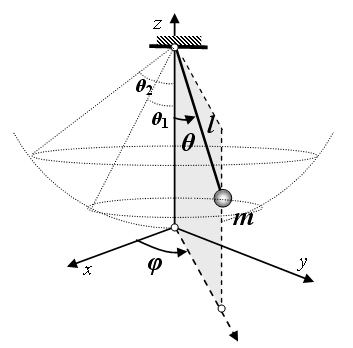
\includegraphics[width=0.5\textwidth]{péndulo_esférico.jpg}
    \caption{Péndulo Esférico.}
    \label{fig:ejemplo}
\end{figure}

\section*{Derivadas temporales}

Como las coordenadas \(x, y, z\) dependen de \(\theta(t)\) y \(\phi(t)\), calculamos las derivadas temporales usando la regla de la cadena y del producto. Tomando las componentes vectoriales de (\ref{Eq1}):

\subsection*{Derivada de \(x(t)\)}

\[
x = l \sin\theta \cos\phi
\]

Aplicamos la derivada:

\[
\dot{x} = \dv{x}{t} = \frac{\partial x}{\partial \theta}\frac{d\theta}{dt} +  \frac{\partial x}{\partial \phi}\frac{d\phi}{dt}= l \left( \cos\theta \cos\phi \, \dot{\theta} - \sin\theta \sin\phi \, \dot{\phi} \right)
\]

Explicación:

\[
\dv{}{t}[\sin\theta \cos\phi] = 
\underbrace{\cos\theta \cos\phi \, \dot{\theta}}_{\text{de } \sin\theta}
-
\underbrace{\sin\theta \sin\phi \, \dot{\phi}}_{\text{de } \cos\phi}
\]

\subsection*{2.Derivada de \(y(t)\)}

\[
y = l \sin\theta \sin\phi
\]

\[
\dot{y} = \dv{y}{t} =\frac{\partial y}{\partial \theta}\frac{d\theta}{dt} +  \frac{\partial y}{\partial \phi}\frac{d\phi}{dt} = l \left( \cos\theta \sin\phi \, \dot{\theta} + \sin\theta \cos\phi \, \dot{\phi} \right)
\]

Explicación:

\[
\dv{}{t}[\sin\theta \sin\phi] = 
\underbrace{\cos\theta \sin\phi \, \dot{\theta}}_{\text{de } \sin\theta}
+
\underbrace{\sin\theta \cos\phi \, \dot{\phi}}_{\text{de } \sin\phi}
\]

\subsection*{3.Derivada de \(z(t)\)}

\[
z = -l \cos\theta
\]

\[
\dot{z} = \dv{z}{t} = \frac{\partial z}{\partial \theta}\frac{d\theta}{dt} = l \sin\theta \, \dot{\theta}
\]

Explicación:

\[
\dv{}{t}[-\cos\theta] = \sin\theta \, \dot{\theta}
\]

Finalmente se obtiene:

\begin{equation}
\begin{aligned}
\dot{x} &= l \cos\theta \cos\phi \, \dot{\theta} - l \sin\theta \sin\phi \, \dot{\phi} \\
\dot{y} &= l \cos\theta \sin\phi \, \dot{\theta} + l \sin\theta \cos\phi \, \dot{\phi} \\
\dot{z} &= l \sin\theta \, \dot{\theta} \\
\dot \vec {r} &= l [(\cos\theta \cos\phi \, \dot{\theta} - l \sin\theta \sin\phi \, \dot{\phi})\hat{x} +
			(\cos\theta \sin\phi \, \dot{\theta} + l \sin\theta \cos\phi \, \dot{\phi})\hat{y} +
			( l \sin\theta \, \dot{\theta})\hat{z}]
\end{aligned}
\label{Eq2}
\end{equation}

\section*{Energía cinética del sistema}

Partimos de las derivadas temporales de las componentes cartesianas de (\ref{Eq2}):

\[
\begin{aligned}
\dot{x} &= l \cos\theta \cos\phi \, \dot{\theta} - l \sin\theta \sin\phi \, \dot{\phi} \\
\dot{y} &= l \cos\theta \sin\phi \, \dot{\theta} + l \sin\theta \cos\phi \, \dot{\phi} \\
\dot{z} &= l \sin\theta \, \dot{\theta}
\end{aligned}
\]

La energía cinética está dada por:

\[
T = \frac{1}{2} m \left( \dot{x}^2 + \dot{y}^2 + \dot{z}^2 \right) = \frac{1}{2}m \dot \vec {r}^{2}
\]

\subsection*{ Cálculo de \(\dot{x}^2\)}

\[
\dot{x} = l (\cos\theta \cos\phi \, \dot{\theta} - \sin\theta \sin\phi \, \dot{\phi})
\]

\[
\dot{x}^{2} = [l (\cos\theta \cos\phi \, \dot{\theta} - \sin\theta \sin\phi \, \dot{\phi})] \cdot [l (\cos\theta \cos\phi \, \dot{\theta} - \sin\theta \sin\phi \, \dot{\phi})]
\]

\[
\dot{x}^2 = l^2 \left( \cos^2\theta \cos^2\phi \, \dot{\theta}^2 - 2 \cos\theta \cos\phi \sin\theta \sin\phi \, \dot{\theta} \dot{\phi} + \sin^2\theta \sin^2\phi \, \dot{\phi}^2 \right)
\]

\subsection*{Cálculo de \(\dot{y}^2\)}

\[
\dot{y} = l (\cos\theta \sin\phi \, \dot{\theta} + \sin\theta \cos\phi \, \dot{\phi})
\]

\[
\dot{y}^{2} = [l (\cos\theta \sin\phi \, \dot{\theta} + \sin\theta \cos\phi \, \dot{\phi})]\cdot[l (\cos\theta \sin\phi \, \dot{\theta} + \sin\theta \cos\phi \, \dot{\phi})]
\]

\[
\dot{y}^2 = l^2 \left( \cos^2\theta \sin^2\phi \, \dot{\theta}^2 + 2 \cos\theta \sin\phi \sin\theta \cos\phi \, \dot{\theta} \dot{\phi} + \sin^2\theta \cos^2\phi \, \dot{\phi}^2 \right)
\]

\subsection*{3. Cálculo de \(\dot{z}^2\)}

\[
\dot{z} = l \sin\theta \, \dot{\theta}
\quad \Rightarrow \quad
\dot{z}^2 = \dot{z}\cdot \dot{z} = [l \sin\theta \, \dot{\theta}] \cdot [l \sin\theta \, \dot{\theta}] =  l^2 \sin^2\theta \, \dot{\theta}^2
\]

\subsection*{4. Suma total: \( \dot{x}^2 + \dot{y}^2 + \dot{z}^2 \)}

Sumamos todas las expresiones anteriores:

\[
\dot{x}^2 + \dot{y}^2 + \dot{z}^2 = l^2 \left[ 
\left( \cos^2\theta \cos^2\phi + \cos^2\theta \sin^2\phi \right) \dot{\theta}^2
+ \left( \sin^2\theta \sin^2\phi + \sin^2\theta \cos^2\phi \right) \dot{\phi}^2 \right.
\]

\[
\left. - 2 \cos\theta \cos\phi \sin\theta \sin\phi \, \dot{\theta} \dot{\phi}
+ 2 \cos\theta \sin\phi \sin\theta \cos\phi \, \dot{\theta} \dot{\phi}
+ \sin^2\theta \, \dot{\theta}^2
\right]
\]

Agrupando:

- Las identidades trigonométricas clave son:

\[
\cos^2\phi + \sin^2\phi = 1
\]

\[
-2 \cos\theta \cos\phi \sin\theta \sin\phi + 2 \cos\theta \sin\phi \sin\theta \cos\phi = 0
\]

Sustituimos y simplificamos:

\[
\dot{x}^2 + \dot{y}^2 + \dot{z}^2 = l^2 \left[ 
\cos^2\theta \cdot 1 \cdot \dot{\theta}^2 + \sin^2\theta \cdot 1 \cdot \dot{\phi}^2 + \sin^2\theta \cdot \dot{\theta}^2 
\right]
\]

\[
= l^2 \left[ (\cos^2\theta + \sin^2\theta) \dot{\theta}^2 + \sin^2\theta \dot{\phi}^2 \right]
\]

\[
= l^2 \left(\dot{\theta}^2 + \sin^2\theta \dot{\phi}^2 \right)
\]

Y finalmente se obtiene:

\begin{equation}
T = \frac{1}{2} m l^2 \left( \dot{\theta}^2 + \sin^2\theta \, \dot{\phi}^2 \right)
\end{equation}
\label{Eq3}

\section*{Energía potencial}

La energía potencial gravitatoria es:

\begin{equation}
V = m g z = -m g l \cos\theta
\end{equation}
\label{Eq4}

\section*{Lagrangiana y ecuaciones de Movimiento}

La Lagrangiana es:

\begin{equation}
\mathcal{L} = T - V = \frac{1}{2} m l^2 \left( \dot{\theta}^2 + \sin^2\theta \, \dot{\phi}^2 \right) + m g l \cos\theta
\label{Eq5}
\end{equation}


\subsection*{Ecuaciones de Euler - Lagrange}

Partimos de la Lagrangiana:

\[
\mathcal{L}(\theta, \phi, \dot{\theta}, \dot{\phi}) = \frac{1}{2} m l^2 \left( \dot{\theta}^2 + \sin^2\theta \, \dot{\phi}^2 \right) + m g l \cos\theta
\]

Aplicamos las ecuaciones de Euler-Lagrange:

\begin{equation}
\dv{t} \left( \pdv{\mathcal{L}}{\dot{q}} \right) - \pdv{\mathcal{L}}{q} = 0
\label{Eq6}
\end{equation}


donde \( q \) es cada coordenada generalizada. Así, introduciendo \((\ref{Eq5})\) en \((\ref{Eq6})\), para cada término se tendrá:

\subsection*{Para \( \theta \)}

Calculamos los términos:

\[
\pdv{\mathcal{L}}{\dot{\theta}} = m l^2 \dot{\theta}
\quad \Rightarrow \quad
\dv{t} \left( \pdv{\mathcal{L}}{\dot{\theta}} \right) = m l^2 \ddot{\theta}
\]

\[
\pdv{\mathcal{L}}{\theta} = m l^2 \sin\theta \cos\theta \, \dot{\phi}^2 - m g l \sin\theta
\]

Por tanto, la ecuación de Lagrange para \( \theta \) es:

\[
m l^2 \ddot{\theta} - m l^2 \sin\theta \cos\theta \, \dot{\phi}^2 + m g l \sin\theta = 0
\]

Simplificamos:

\begin{equation}
\boxed{
\ddot{\theta} - \sin\theta \cos\theta \, \dot{\phi}^2 + \frac{g}{l} \sin\theta = 0
}
\label{Eq7}
\end{equation}

\subsection*{Para \( \phi \)}

Calculamos los términos:

\[
\pdv{\mathcal{L}}{\dot{\phi}} = m l^2 \sin^2\theta \, \dot{\phi}
\quad \Rightarrow \quad
\dv{t} \left( \pdv{\mathcal{L}}{\dot{\phi}} \right)
= m l^2 \left( 2 \sin\theta \cos\theta \, \dot{\theta} \dot{\phi} + \sin^2\theta \, \ddot{\phi} \right)
\]

\[
\pdv{\mathcal{L}}{\phi} = 0
\]

Por tanto, la ecuación de Lagrange para \( \phi \) es:

\[
m l^2 \left( 2 \sin\theta \cos\theta \, \dot{\theta} \dot{\phi} + \sin^2\theta \, \ddot{\phi} \right) = 0
\]

Simplificamos:

\begin{equation}
\boxed{
\sin^2\theta \, \ddot{\phi} + 2 \sin\theta \cos\theta \, \dot{\theta} \dot{\phi} = 0
}
\label{Eq8}
\end{equation}

También se puede escribir como:

\begin{equation}
\boxed{
\ddot{\phi} + 2 \cot\theta \, \dot{\theta} \dot{\phi} = 0
}
\label{Eq9}
\end{equation}

\subsection*{Ecuaciones de movimiento obtenidas}

\begin{equation}
\boxed{
\ddot{\theta} - \sin\theta \cos\theta \, \dot{\phi}^2 + \frac{g}{l} \sin\theta = 0
\quad , \quad
\ddot{\phi} + 2 \cot\theta \, \dot{\theta} \dot{\phi} = 0
}
\label{Eq10}
\end{equation}

\section*{Aproximación para ángulos pequeños}

Cuando los ángulos \( \theta \) y \( \phi \) son pequeños (\( \theta, \phi \ll 1 \)), se pueden aplicar las siguientes aproximaciones trigonométricas:

\[
\sin\theta \approx \theta, \qquad \cos\theta \approx 1, \qquad \cot\theta \approx \frac{1}{\theta}
\]

Partimos de las ecuaciones de Lagrange del péndulo esférico:

\[
\begin{aligned}
\ddot{\theta} - \sin\theta \cos\theta \, \dot{\phi}^2 + \frac{g}{l} \sin\theta &= 0 \\
\ddot{\phi} + 2 \cot\theta \, \dot{\theta} \dot{\phi} &= 0
\end{aligned}
\]

\subsection*{Primera ecuación: \( \theta \)}

Aplicando las aproximaciones:

\[
\sin\theta \cos\theta \approx \theta, \qquad \sin\theta \approx \theta
\]

Entonces:

\[
\ddot{\theta} - \theta \, \dot{\phi}^2 + \frac{g}{l} \theta = 0
\]

\begin{equation}
\boxed{
\ddot{\theta} + \left( \frac{g}{l} - \dot{\phi}^2 \right) \theta = 0
}
\label{Eq11}
\end{equation}

Esto representa una ecuación diferencial lineal para pequeñas oscilaciones, similar a un péndulo simple, pero con una frecuencia angular \((g/l)\), modificada por el llamado término centrífugo \( \dot{\phi}^2 \).

\subsection*{Segunda ecuación: \( \phi \)}

Usamos la aproximación:

\[
\cot\theta \approx \frac{1}{\theta}
\]

Entonces:

\begin{equation}
\ddot{\phi} + 2 \frac{1}{\theta} \dot{\theta} \dot{\phi} = 0
\quad \Rightarrow \quad
\boxed{
\ddot{\phi} + 2 \frac{\dot{\theta}}{\theta} \dot{\phi} = 0
}
\label{Eq12}
\end{equation}

Esta ecuación es aún no lineal, pero si se asume que \( \theta \) es constante (por ejemplo, \( \dot{\theta} \approx 0 \)), entonces:

\begin{equation}
\boxed{
\ddot{\phi} \approx 0 \quad \Rightarrow \quad \dot{\phi} = \text{constante}
}
\label{Eq13}
\end{equation}

\subsection*{Conclusiones}

En el límite de ángulos pequeños:

\begin{itemize}
    \item Las ecuaciones se simplifican considerablemente y pueden tratarse como lineales.
    \item El movimiento en \( \theta \) se asemeja al de un péndulo simple, pero afectado por la velocidad angular \( \dot{\phi} \).
    \item El movimiento en \( \phi \) se desacopla parcialmente, y en ciertos casos puede considerarse uniforme.
\end{itemize}

\end{document}